\documentclass[xcolor=dvipsnames, compress]{beamer}
%\usetheme{Madrid} % My favorite!
%\usetheme{Boadilla} % Pretty neat, soft color.
%\usetheme{Warsaw}
%\usecolortheme{dove} 
%\usetheme[secheader]{Boadilla}
%\useoutertheme[subsection=false]{smoothbars}
% \useinnertheme{rectangles}
% \usetheme{Marburg}
%   \usecolortheme[RGB={139,10,80}]{structure}
%  \usecolortheme[RGB={25,25,112}]{structure}
%\usecolortheme[RGB={255,127,36}]{structure}
\usetheme{CambridgeUS}
%\usetheme{PaloAlto}
% \usefonttheme{professionalfonts}
% \usepackage{listings}

%\usetheme{Boadilla}

% \usetheme{Warsaw}
%\usetheme{Darmstadt} %OK!
%  \usetheme{Frankfurt} %OK!
% \usetheme{Goettingen}
% \usetheme{Dresden}
%\usetheme{JuanLesPins} %OK!!
%\usetheme{Marburg}
%  \usetheme{Montpellier}
% \usetheme{Rochester} %sobrio
%\usetheme{Singapore}
%\usetheme{Szeged}
%\usetheme{Luebeck}

%\usetheme{Hannover}
%\usecolortheme{wolverine}

%\usecolortheme{albatross}
%\usecolortheme{seahorse}
%\usecolortheme{beetle}
%\usecolortheme{crane}
%\usecolortheme{dolphin}
%\usecolortheme{dove} %<- este con orchid
%\usecolortheme{fly}
%\usecolortheme{lily}
%\usecolortheme{orchid}
%\usecolortheme{rose}
%\usecolortheme{seagull}
%\usecolortheme{whale}

%\usetheme{Bergen} % This template has nagivation on the left
%\usetheme{Frankfurt} % Similar to the default 
%with an extra region at the top.
%\usecolortheme{seahorse} % Simple and clean template
%\usetheme{Darmstadt} % not so good
% Uncomment the following line if you want %
% page numbers and using Warsaw theme%
% \setbeamertemplate{footline}[page number]
%\setbeamercovered{transparent}
%\setbeamercovered{invisible}
% To remove the navigation symbols from 
% the bottom of slides%
%\setbeamertemplate{navigation symbols}{} 
%
\usepackage{graphicx}
\usepackage{amssymb,amsmath,amscd}
\usepackage{latexsym,xspace}
\usepackage[utf8]{inputenc}
\usepackage{epsfig}
%\usepackage{fancyhdr}
%\usepackage[spanish]{babel}
\usepackage[all]{xy}
\usepackage{enumerate}
\usepackage{eucal}
%\usepackage[usenames]{color}

\usepackage{mathtools} % flechas con nombres arriba o abajo


%#########################
\newcommand{\tx}{\ensuremath{\tau(X)}}
\newcommand{\txx}{\ensuremath{\tau_{X}}}
\newcommand{\Q}{\ensuremath{\mathbb{Q}}}
\newcommand{\Z}{\ensuremath{\mathbb{Z}}}
\newcommand{\N}{\ensuremath{\mathbb{N}}}
\newcommand{\R}{\ensuremath{\mathbb{R}}}
\newcommand{\C}{\ensuremath{\mathbb{C}}}
\newcommand{\A}{\ensuremath{\forall}}
\newcommand{\E}{\ensuremath{\exists}}
\newcommand{\iso}{\ensuremath{\cong}}
\newcommand{\union}{\ensuremath{\cup}}
%\newcommand{\morinyec}{\ensuremath{\precapprox}}
%\newenvironment{prueba}{\vspace{-3mm}\noindent\textbf{Demostraci\'on}\\}{\noindent$\blacksquare$\\}
\newcommand{\nin}{\ensuremath{\notin}}
\renewcommand{\emptyset}{\varnothing}

%\newcommand{\niso}{\ensuremath{\not \cong}}
\newtheorem{teor}{Teorema}[section]
\newtheorem{defi}{Definition}[section]
\newtheorem{ejemplo}{Examples}[section]
\newtheorem{obs}{Remark}[section]
\newtheorem{prop}{Proposition}[section]
\newtheorem{cor}{Corollary}[section]
\newtheorem{ntc}{Notation}[section]
\newtheorem{lema}{Lemma}[section]
\newtheorem{prob}{Problem}
\newtheorem{comen}{Comment}


%\usepackage{bm}         % For typesetting bold math (not \mathbold)
%\logo{\includegraphics[height=0.6cm]{yourlogo.eps}}
%
\title[Aprendizaje de Máquina y Cobertura BAF]{M\'etodos de aprendizaje de maquina para inferir el nivel de cobertura de banda ancha fija en municipios de M\'exico}
\author{César Zamora Martínez}
\institute[ITAM]
%\date{Diciembre 16, 2019}
% \today will show current date. 
% Alternatively, you can specify a date.
%


\begin{document}
%
\begin{frame}
\titlepage
\end{frame}

\begin{frame}
\frametitle{Índice}
 \tableofcontents%[sections]
\end{frame}

%\begin{frame}
%\section{Cobertura de banda ancha fija en México}
%\frametitle{¿Cómo funciona el Internet?}
%Internet es red muy compleja y extensa donde muchas redes se interconectan para mandar información entre sus nodos.
%\begin{figure}
%	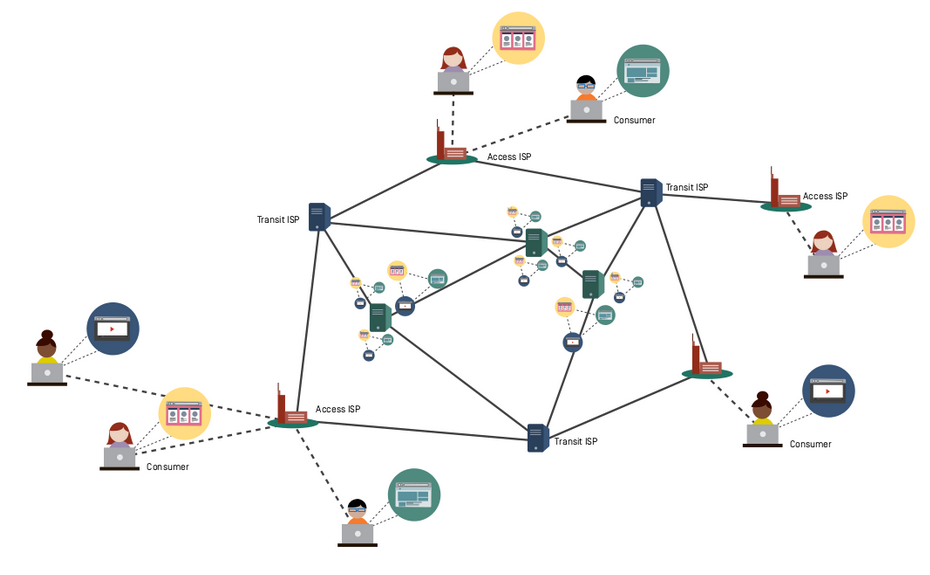
\includegraphics[scale=0.3]{images/internet_diagram.png}
%	%\caption{Insertando imagen}
%\end{figure}
%\end{frame}
%
%\begin{frame}
%\frametitle{¿Cómo funciona el Internet?}
%Los operadores hacen \textbf{inversiones considerables} en equipo e infraestructura para conectar a los usuarios y manejar el tráfico sobre sus redes.
%\begin{figure}
%	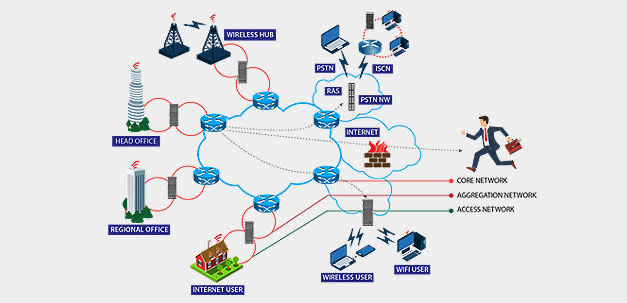
\includegraphics[scale=0.5]{images/core_network.jpg}
%	%\caption{Insertando imagen}
%\end{figure}
%\end{frame}

\begin{frame}
\section{Cobertura de banda ancha fija en México}
\frametitle{Velocidad y red de acceso}
\begin{figure}
	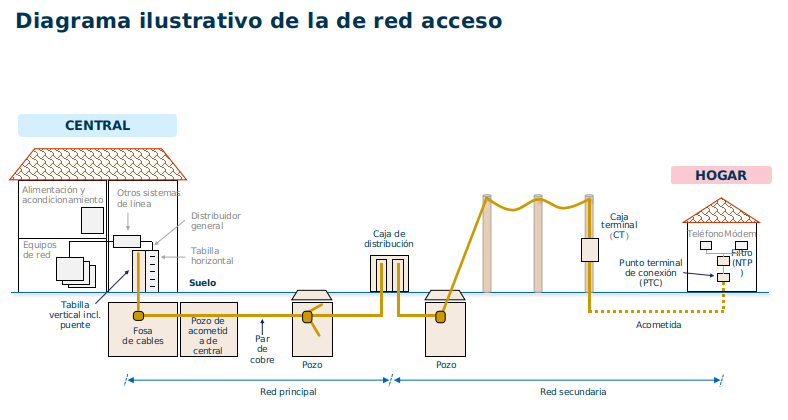
\includegraphics[scale=0.43]{images/access_network.jpg}
	%\caption{Insertando imagen}
\end{figure}
\end{frame}

\begin{frame}
\frametitle{Velocidad y red de acceso}
La velocidad de Internet se encuentra limitada, por la tecnología de acceso. 

\begin{figure}
	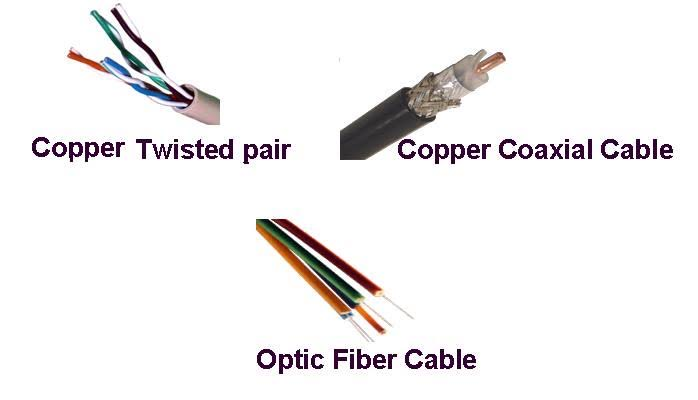
\includegraphics[scale=0.2]{images/access_technology.jpg}
	%\caption{Insertando imagen}
\end{figure}

\begin{block}{Interés de este trabajo}
	Cobertura de cable coaxial y fibra óptica (alta velocidad); requiere grandes inversiones; solo se despliegan en zonas densamente pobladas o con recursos.
\end{block}

\end{frame}

\begin{frame}
\frametitle{¿Cómo está México en cobertura de banda ancha fija?}

\begin{itemize}
	
\item México: 18.9 millones. de accesos + 120 millones de habitantes.
\item Accesos: $22\%$ fibra + $37\%$ cable coaxial (total $59\%$)

\item OCDE, proxy de los suscriptores de BAF por cada 100 habitantes la región \footnote{http://www.oecd.org/internet/broadband/broadband-faqs.htm}:
\begin{equation}\label{pen_habitantes}
\mbox{ Accesos por cada 100 habitantes } = \frac{Accesos }{Habitantes} \times 100 
\end{equation}
\end{itemize}

\end{frame}

\begin{frame}

\begin{figure}
	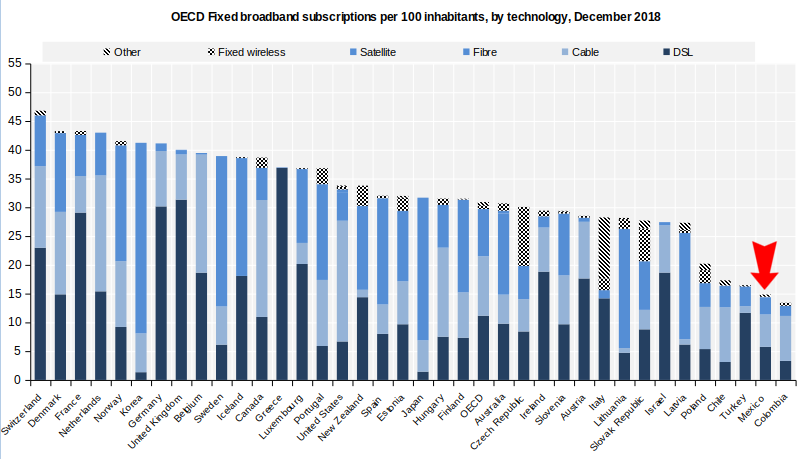
\includegraphics[scale=0.4]{images/ocde.png}
	%\caption{Insertando imagen}
\end{figure}
\end{frame}


 \begin{frame}
\frametitle{¿Cómo está México en cobertura de banda ancha fija?}
\begin{itemize}
	\item En México hay 2,457 municipios,
	\item ¿cómo se ve la cobertura de fibra óptica y cable coaxial en ellos? 
	\item Veamos el mapa (Junio 2019).
	\item Cobertura municipal: dependemos de mucha información de operadores que no siempre está disponible (públicamente)  o actualizada
	\item ¿Se puede inferir el nivel de cobertura con información alterna?	
\end{itemize}
\end{frame}

\begin{frame}
\section{Problemas a explorar}
\frametitle{Problemas de clasificación de cobertura}

A  nivel municipal...

\begin{itemize}
	\item[\textbf{P1:}] ¿Existe o no penetración de BAF de fibra óptica o cable coaxial?
	\item[\textbf{P2:}] ¿Cuál es el nivel de penetración de BAF de fibra óptica o cable coaxial?
\end{itemize}

\begin{figure}
	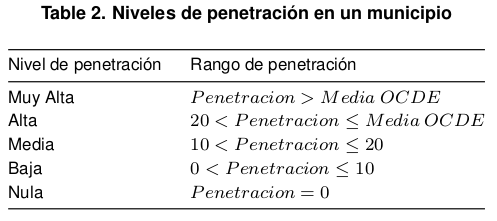
\includegraphics[scale=0.5]{images/ocde_class.jpg}
	%\caption{Insertando imagen}
\end{figure}

\end{frame}

\begin{frame}
\frametitle{Ideas}
\begin{columns}
	\begin{column}{0.5\textwidth}  %%<--- here
		\textbf{Información socio-demográfica de municipios:}
		\begin{itemize}
			\item Encuesta Intercensal 2015 (INEGI),
			\item Información de índice de marginación 2015 (CONAPO)
			\item Accesos por tecnología, Junio 2019 (IFT)
			\item Ingreso per cápita "Índice de Desarrollo Humano" (PNUD-ONU)
		\end{itemize}
		
	\end{column}
	\begin{column}{0.5\textwidth}
		\textbf{Pipeline:}
		\begin{itemize}
			\item Modelos: Regresión logística, Random Forest, Gradient Tree Bost
			\item Gridsearch, calibrar los posibles hiper-parámetros de los modelos + validación cruzada,
			\item Comparar modelos,
			\item Analizar los resultados	
		\end{itemize}


	\end{column}
\end{columns}

\end{frame}



\begin{frame}
\frametitle{Ideas}
\begin{columns}
	\begin{column}{0.5\textwidth}  %%<--- here
		\textbf{P1 - Variables principales :}
		\begin{itemize}
			\item hogares, habitantes
			\item $hogares/km^2$, $habitantes/km^2$
			\item \% hogares sin acceso a energía eléctrica
			\item \% pob. en localidades de menos de 5,000 habitantes
			\item Ingreso promedio anual per cápita
			\item Habs. que gana menos de 2 SMM,
			\item \% hogs con servicios tv paga + teléfono fijo + celular
		\end{itemize}
		
	\end{column}
	\begin{column}{0.5\textwidth}
		\textbf{Pipeline:}
		\begin{itemize}
			\item Modelos: Regresión logística, Random Forest, Gradient Tree Bost
			\item Gridsearch, calibrar los posibles hiper-parámetros de los modelos + validación cruzada,
			\item Comparar modelos,
			\item Analizar los resultados	
		\end{itemize}
		
		
	\end{column}
\end{columns}

\end{frame}


%
%\begin{frame}[fragile] % Notice the [fragile] option %
%\frametitle{Verbatim}
%\begin{example}[Putting Verbatim]
%\begin{verbatim}
%\begin{frame}
%\frametitle{Outline}
%\begin{block}
%{Why Beamer?}
%Does anybody need an introduction to Beamer?
%I don't think so.
%\end{block}
% Extra carriage return causes problem with verbatim %
%\end{frame}\end{verbatim} 
%\end{example}
%\end{frame}
 
%\begin{frame}[fragile]  % notice the fragile option, since the body
			% contains a verbatim command
%Example of the \verb|\cite| command to give a reference is below:
%Example of citation using \cite{key1} follows on.
%\end{frame}
 
% \begin{frame}
% \section{Bibliografía}
% \frametitle{Referencias}
% \footnotesize{
% \begin{thebibliography}{99}
%  \bibitem[Morita, 2010]{key1} J. Nagata, K. Morita (1989)
%  \newblock Topics On General Topology.
%  \newblock \emph{Elsevier Science Publisher B.V.} 15(6), 203 -- 243.

% \bibitem[VanMill, 2010]{key1} J. Van Mill ; M. Husek (1992)
%  \newblock Recent Progress In General Topology.
%  \newblock \emph{Elsevier Publications} p. 375.

% \bibitem[MacLane, 2010]{key1} J. S. Mac Lane(1971)
%  \newblock Categories for the working mathematician,.
%  \newblock \emph{Springer} p. 375.

%  \bibitem[Ishii, 2010]{key1} Tadashi Ishii (1969)
%  \newblock On Tychonoff Functor and $w$-Compactness.
%  \newblock \emph{Topology Appl.} 11, 175 -- 187.

%  \bibitem[Ishii, 2010]{key1} T. Hoshina; K. Morita (1980)
%  \newblock On Regular Products Of Topological Spaces.
%  \newblock \emph{Topology Appl.} 11, 47 -- 57.
% \end{thebibliography}
% }
% \end{frame}


 
% \begin{frame}
% %\section{Bibliografía}
% \frametitle{Referencias}
% \footnotesize{
% \begin{thebibliography}{99}
%  \bibitem[Porter, 2010]{key1}J. R. Porter ; R. Grant Woods  (1987)
%  \newblock Extensions and Absolutes of Hausdorff Spaces.
%  \newblock \emph{Springer-Verlag} 856.


%  \bibitem[Simon, 2010]{key1} Petr Simon (1984)
%  \newblock Completely regular modification and products.
%  \newblock \emph{Commentationes Mathematicae Universitatis Carolinae} 25(1), 121--128.



%  \bibitem[Puppier, 2010]{key1} René Puppier (1969)
%  \newblock La Completion Universelle D'un Produit D'espaces Completement Reguliers .
%  \newblock \emph{Publ. Dept. Math, Lyon} 254, 342--351.



% \end{thebibliography}
% }
% \end{frame}
% 
% End of slides
\end{document} 